\documentclass[times, utf8, seminar]{fit}

%\batchmode
%\usepackage{booktabs}
\usepackage{listings}
\usepackage{longtable}
\usepackage{xcolor}
\usepackage{float}
\usepackage{enumitem}
\usepackage{hyperref}
\usepackage{enumerate}
\usepackage{graphicx}
\usepackage{etoolbox}
\usepackage{datetime}
\usepackage{needspace}
\usepackage{titlesec}
%\titleformat{\chapter}[display]{\normalfont\huge\bfseries}{\chaptertitlename\ \thechapter}{20pt}{\Huge}

\begin{document}
\widowpenalty=300
\clubpenalty=300

\lstset{
  language=bash,
  backgroundcolor=\color{gray!25},
  basicstyle=\ttfamily \footnotesize,
  breaklines=true,
  prebreak=\raisebox{0ex}[0ex][0ex] \hookleftarrow,
  columns=fullflexible
}


% this alters "before" spacing (the second length argument) to 0
%\titlespacing*{\chapter}{0pt}{0pt}{40pt}

% this changes "before" spacing back to its default of 50pt
%\titlespacing*{\chapter}{0pt}{50pt}{40pt}}

%\titlespacing*{\chapter}{0pt}{-50pt}{18pt}
%\titleformat{\chapter}[display]{\normalfont\huge\bfseries}{\chaptertitlename\ \thechapter}{20pt}{\Huge}

\title{Agilni softver inžinjering}

\author{Ernad Husremović}
\brindex{DL 2792}
\verzija {0.0.1}

\mentor{mr. Adil Joldić}

\maketitle

\tableofcontents

%\listoftables
%\listoffigures
\newpage

% abstract begin
%\begin{abstract}
%
%To be done 
%
%\keywords{open source software, OSS, Bosna i Hercegovina}
%\end{abstract}

% abstract end

\chapter{Uvod}
\vspace*{-0.7cm}

Šta znači `biti agilan'?

Agilni razvoj software-a ne predstavlja specifični proces. Agilni razvoj je način na koji se razmišlja o razvoju software-a\citep{agileart}\citep[str. 9]{agileart}.

Osnovna polazišta ovog načina razmišljanja opisuje "Agilni manifest"\footnote{\url{http://agilemanifesto.org/iso/en/principles.html}}, koji je definisan kroz četiri vrijednosti i 12 principa:

Vrijednosti:
\begin{itemize}
\item Ljudi i interakcije ispred procesa i alata
\item Software koji funkcioniše ispred iscrpne dokumentacije
\item Komunikacija sa klijentima ispred pregovora
\item Odgovor na promjene ispred slijeđenja plana
\end{itemize}

Principi:
\begin{itemize}
\item Glavni prioritet je zadovoljiti zahtjeve klijente kroz ranu i kontinuiranu \emph{isporuku} software-a
\item Blagonaklono prihvatiti \emph{promjene} funkcionalnih zahtjeva, čak i u kasnijim fazama razvoja.
\item Funkcionalan software treba isporučivati \emph{često}, nakon par hefti ili mjeseci, nastojeći da taj period bude što kraći.
\item Najefikasniji način razmejene informacija unutar razvojnog tima je direktna - `face-to-face' komunikacija.
\item Software koji \emph{funkcioniše} je primarna mjera uspjeha projekta.
\item Agilni procesi promoviraju održivi razvoj. Finansijeri, developeri i korisnici trebaju biti u stalnoj koordinaciji, bez obzira na dužinu trajanja projekta.
\item Kontinuirano pažnja na \emph{kvalitet} tehničkih operacije i dobar dizajn povećava agilnost.
\item \emph{Jednostavnost}, kao vještina postizanja maksimalnog učinka sa što manje rada, je krucijalni agilni princip.
\item Najbolja arhitektura, funkcionalni zahtjevi i dizajn se postižu u \emph{samo-organizovanim} timovima.
\item Tim redovno analizira predhodne operacije u cilju bolje efektivnosti (\emph{refleksija}). Na osnovu tih rezultata, tim podešava i koriguje buduće operacije.
\end{itemize}



\chapter{Analiza}
\vspace*{-0.7cm}

\section{Test}

\begin{figure}[H]
\centering
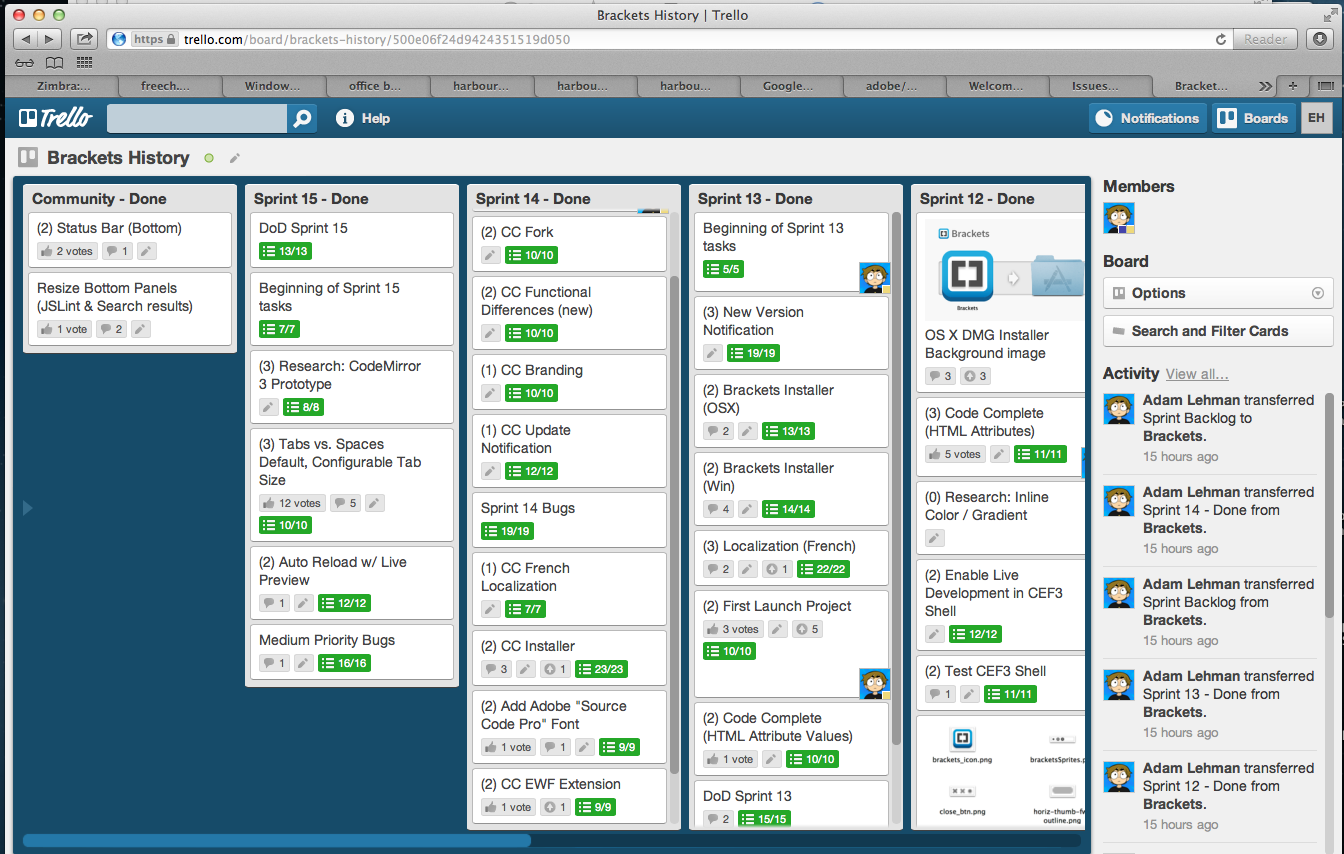
\includegraphics[width=10cm]{img/brackets_trello_sprint_history.png}
\caption{trello}
\end{figure}

\section{Git}

Git je tito.

\subsection{Git merge from upstream}

gitlabhq\$ git fetch gitlabhq

\begin{lstlisting}
remote: Counting objects: 570, done.
remote: Compressing objects: 100\% (174/174), done.
remote: Total 342 (delta 262), reused 237 (delta 165)
Receiving objects: 100\% (342/342), 43.70 KiB, done.
Resolving deltas: 100\% (262/262), completed with 122 local objects.
From git://github.com/gitlabhq/gitlabhq
   dd4d124..3c7806c  master     -> gitlabhq/master
\end{lstlisting}


gitlabhq\$ git branch -l

\begin{lstlisting}
* master
\end{lstlisting}


gitlabhq\$ git commit -a

\begin{lstlisting}
[master 9bacff4] http://www.quora.com/Ruby-on-Rails/What-is-schema-rb-in-rails-project
 1 file changed, 19 insertions(+), 19 deletions(-)
\end{lstlisting}



gitlabhq\$ git diff HEAD\^1 HEAD

\begin{lstlisting}
diff --git a/db/schema.rb b/db/schema.rb
index 51ab207..19eb8eb 100644
--- a/db/schema.rb
+++ b/db/schema.rb
@@ -69,8 +69,8 @@ ActiveRecord::Schema.define(:version => 20121026114600) do
     t.boolean  "closed",                              :default => false, :null => false
     t.datetime "created_at",                                             :null => false
     t.datetime "updated_at",                                             :null => false
-    t.text     "st_commits",    :limit => 2147483647
-    t.text     "st_diffs",      :limit => 2147483647
+    t.text     "st_commits",    :limit => 4294967295

  ...

     t.integer  "project_id"
     t.string   "attachment"
     t.string   "line_code"
@@ -156,30 +156,30 @@ ActiveRecord::Schema.define(:version => 20121026114600) do
   end
 
   create_table "users", :force => true do |t|
\end{lstlisting}


gitlabhq\$ git merge gitlabhq/master

\begin{lstlisting}
Removing lib/gitlab/encode.rb
Removing gitlab
Auto-merging doc/development.md
Removing Procfile.production
Merge made by the recursive strategy
 .travis.yml                                        |    2 +-
 CHANGELOG                                          |    2 +-
 Gemfile                                            |    4 +-
 Gemfile.lock                                       |   12 +++-
 Procfile.production                                |    2 -
 VERSION                                            |    2 +-
 app/assets/images/event_filter_comments.png        |  Bin 0 -> 750 bytes
 app/assets/images/event_filter_merged.png          |  Bin 0 -> 463 bytes
 app/assets/images/event_filter_push.png            |  Bin 0 -> 632 bytes
 
 ...

 app/controllers/application_controller.rb          |    9 +++
 app/controllers/blob_controller.rb                 |   10 +--
 app/controllers/dashboard_controller.rb            |   11 ++-
 app/controllers/profile_controller.rb              |    2 +-

 ...

 app/views/blame/show.html.haml                     |    4 +-
 app/views/commits/_commit.html.haml                |    4 +-
 app/views/commits/_head.html.haml                  |    5 ++
 app/views/dashboard/index.html.haml                |    9 ++-
 
 ... 
 
 delete mode 100644 Procfile.production
 create mode 100644 app/assets/images/event_filter_comments.png
 create mode 100644 app/assets/images/event_filter_merged.png
 create mode 100644 app/assets/images/event_filter_push.png
 ...
 delete mode 100644 lib/gitlab/encode.rb
 create mode 100644 lib/gitlab/git_stats.rb
 create mode 100644 vendor/assets/javascripts/g.bar-min.js
 create mode 100644 vendor/assets/javascripts/g.raphael-min.js
\end{lstlisting}



gitlabhq\$ git push origin master

\begin{lstlisting}
Counting objects: 581, done.
Delta compression using up to 8 threads.
Compressing objects: 100\% (85/85), done.
Writing objects: 100\% (350/350), 45.00 KiB, done.
Total 350 (delta 267), reused 342 (delta 262)
To git@github.com:hernad/gitlabhq.git
   038ac96..28f5807  master -> master

\end{lstlisting}



%\begin{center}
%\emph{\large{Freedom to create, distribute, and use open source software (OSS).}}
%\end{center}

\chapter {Gitlab}
\vspace*{-0.7cm}

\section{Source control}

\section{Issues}

\section{Wiki}

\chapter{Zaključak}

.

% -------------------------------------------------
\bibliography{literatura}
\bibliographystyle{fit}

% -------------------------------------------------
\appendix

\chapter{Instalacija}
\vspace*{-0.7cm}
\setlength{\parindent}{0cm}
%\setlength{\parindent}{default}

\chapter{Software toolset}
\begin{enumerate}
  \item Mac OS X 10.8.2
  \item mvim, vim tekst editor ver 7.3
  \item MacTex (TeX Live 2012)
\end{enumerate}

\chapter{Software repozitoriji}

\begin{itemize}
  \item Agilni developerski environment  \url{https://github.com/hernad/atile\_dev\_env}

\end{itemize}

\end{document}
